\chapter{One-loop neutrino masses}
Here we calculate the one-loop neutrino mases in the mass-basis

\section{Extra particles}
We assume to have $\alpha$-scalar and $n$-fermions with the mass-eigenstate couplings (Weyl spinors)
\begin{align}
  \mathcal{L}=\left(y_{in\alpha}\nu_{i}\chi_n S_{\alpha}+y'_{mi\alpha}\chi_n\nu_{i} S_{\alpha}^{\dagger}+\text{h.c}+m_n \chi_n\chi_n  \right)+m_{\alpha}^2\,S_{\alpha}^2+
\end{align}
From left to right in Figure~\ref{fig:1lnu}
\begin{figure}
  \centering
  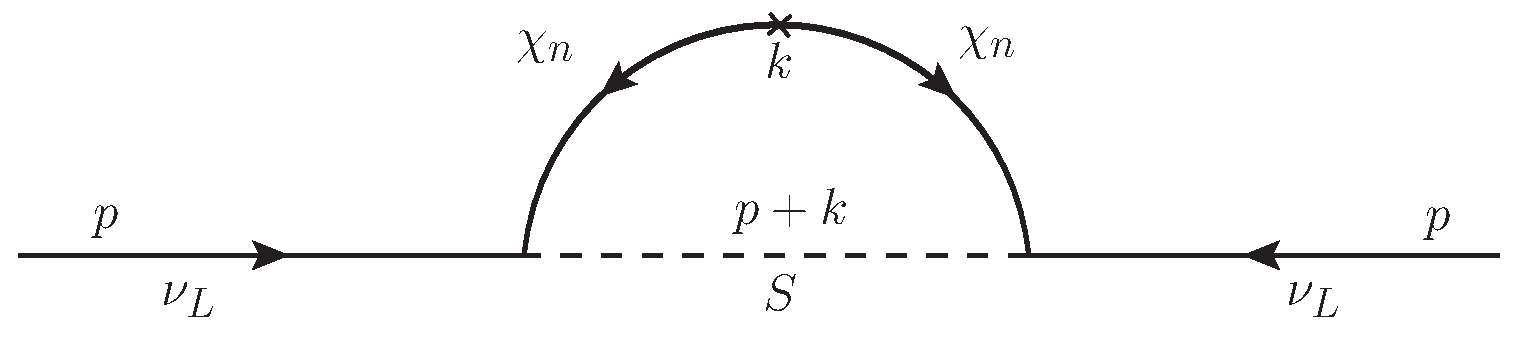
\includegraphics[scale=0.5]{onelooopneutrino}
  \caption{Generic one-loop neutrino mass contribution}
  \label{fig:1lnu}
\end{figure}
\begin{align}
-i\Sigma^{\nu}_{ij}(p)=&\int \frac{d4k}{\left( 2\pi \right)^{4}}\left(y_{in\alpha}  \right)iS_F(k) \left(y_{jn\alpha}\right)i\Delta_F(p+k) \nonumber\\
=&\frac{y_{i n\alpha}y_{j n\alpha}}{16\pi^2}\int \frac{d^4k}{i\pi^2}\frac{\cancel{k}+m_{\chi_n}}{\left(k^2-m_{\chi_n}^2  \right)\left[\left(p+k\right)^2-m_{S_\alpha}^2\right]}
\end{align}
In the limit $p\to 0$
\begin{align}
\label{eq:mnub0}
   M^{\nu}_{ij}=&-\frac{y_{i n\alpha}y_{j n\alpha}}{16\pi^2}m_{\chi_n} B_0 \left( 0;m_{\chi_n}^2,m_{S_{\alpha}}^2 \right) \,.
\end{align}
where $B_0\left
(0;m_{\chi_n}^2,m^2_{S_{\alpha}} \right)$ is the $B_0$ Passarino-Veltman function~\cite{Passarino:1978jh}

\begin{align*}
  B_0 \left(0;m_{\chi_n}^2,m^2_{S_{\alpha}} \right)=&\int \frac{d^4k}{i\pi^2}\frac{1}{\left(k^2-m_{\chi_n}^2\right)\left(k^2-m_{S_\alpha}^2\right)}\nonumber\\
            =&\frac{1}{m_{\chi_n}^2-m_{S_\alpha}^2}\left[ A_0\left(m_{\chi_n}^2\right)-A_0\left(m_{S_\alpha}^2\right)  \right],
\end{align*}
and
\begin{align*}
  A_0\left(m^2\right)=m^2 \left[ \Delta+1-\ln \left( m^2/\mu^2 \right) \right]
\end{align*}
with
\begin{align*}
  \Delta=\left( \frac{2}{\epsilon}-\ln\pi+\gamma_E \right),
\end{align*}
where $\mu$ is the subtraction point (dimensional regularization) an $\gamma_E$ is the Euler-Mascheroni constant.
Replacing back in eq.~\eqref{eq:mnueig}, we have
\begin{align}
   B_0 \left(0;m_{\chi_n}^2,m^2_{S_{\alpha}} \right)=&
   \frac{1}{m_{\chi_n}^2-m_{S_\alpha}^2}\left[m^2_{\chi_n} \left[ \Delta+1-\ln \left( m_{\chi_n}^2/\mu^2 \right) \right]  \right] 
-m_{S_\alpha}^2 \left[ \Delta+1-\ln \left( m_{S_\alpha}^2/\mu^2 \right) \right] \nonumber\\
=&(\Delta+1)+\frac{m_{S_\alpha}^2\ln \left( m_{S_\alpha}^2/\mu^2 \right)-m_{\chi_n}^2\ln \left( m_{\chi_n}^2/\mu^2 \right)}{m_{\chi_n}^2-m_{S_\alpha}^2} \nonumber\\
=&\left[\Delta+1+\ln\left( \mu^2 \right) \right]+\frac{m_{S_\alpha}^2\ln \left( m_{S_\alpha}^2 \right)-m_{\chi_n}^2\ln \left( m_{\chi_n}^2 \right)}{m_{\chi_n}^2-m_{S_\alpha}^2} \nonumber\\
=&\operatorname{cte}(\infty)+\frac{m_{S_\alpha}^2\ln \left( m_{S_\alpha}^2 \right)-m_{\chi_n}^2\ln \left( m_{\chi_n}^2 \right)}{m_{\chi_n}^2-m_{S_\alpha}^2} \,.
\end{align}
Reemplazando en eq.~\eqref{eq:mnub0}:

\begin{align}
 M^{\nu}_{ij}=&-\frac{y_{i n\alpha}y_{j n\alpha}}{16\pi^2}m_{\chi_n} \left[ \operatorname{cte}(\infty)+
f \left( m_{\chi_n},m_{S_{\alpha}} \right) \right] \,,
\end{align}
where
\begin{align}
f \left( m_{\chi_n},m_{S_{\alpha}} \right)=&  
\frac{m_{S_{\alpha}}^2\ln \left(m_{S_{\alpha}}^2\right)-m_{\chi_n}^2\ln \left(m_{\chi_n}^2  \right)}{m_{\chi_n}^2-m_{S_{\alpha}}^2}
\end{align}

\section{Applications}

\section{Singlet-doublet fermions with scalar singlets}
There~\cite{Restrepo:2015ura}

\begin{align}
  y_{i n\alpha}=&h_{i\alpha}N_{3n} 
\end{align}
and 
\begin{align}
   M^{\nu}_{ij}=&\sum_{\alpha}\frac{h_{i\alpha}h_{j\alpha}}{16\pi^2}\sum_{n=1}^3 \left( N_{3n} \right)^2m_{\chi_n}
\,f\left( m_{S_\alpha},m_{\chi_n} \right).
\end{align}

\subsection{Zee}

In the Zee model we can work in the Higgs-basis with $\left\langle H_1 \right\rangle=v/\sqrt{2}$,  $\left\langle H_2 \right\rangle=0$ \cite{AristizabalSierra:2006ri}. In that basis the scalar potential is
\begin{align}
  \label{eq:scalarpotentialinhiggsbas}
  V  = & \mu^{2}_{1}H_{1}^{\dagger}H_{1}
  + \mu^{2}_{2}H_{2}^{\dagger}H_{2}
  - [\mu^{2}_{3}H_{1}^{\dagger}H_{2} + \mbox{H.c.}]
  + \frac{1}{2}\lambda_{1}(H_{1}^{\dagger}H_{1})^{2}
  \nonumber\\
  & + \frac{1}{2}\lambda_{2}(H_{2}^{\dagger}H_{2})^{2}
  + \lambda_{3}(H_{1}^{\dagger}
  H_{1})(H_{2}^{\dagger}H_{2})
  + \lambda_{4}(H_{1}^{\dagger}
  H_{2})(H_{2}^{\dagger}H_{1})
  \nonumber\\
  & + \left\{
    \frac{1}{2}\lambda_{5}(H_{1}^{\dagger}H_{2})^{2}
    + [\lambda_{6}(H_{1}^{\dagger}H_{1})
    + \lambda_{7}(H_{2}^{\dagger}H_{2})]
    H_{1}^{\dagger}H_{2}
    +\mbox{H.c.}
  \right\}
  \nonumber\\
  & + \mu_{h}^{2}|h^{+}|^{2} + \lambda_{h}|h^{+}|^{4}
  + \lambda_{8}|h^{+}|^{2}H_{1}^{\dagger}H_{1} 
  + \lambda_{9}|h^{+}|^{2}H_{2}^{\dagger}H_{2}
  \nonumber\\
  & + \lambda_{10}|h^{+}|^{2}(H_{1}^\dagger H_{2}
  + \mbox{H.c.})
  + \mu\epsilon_{\alpha\beta}H_{1}^{\alpha}
  H_{2}^{\beta}h^{-}.
\end{align}

We define
\begin{align}
  H_1=&
  \begin{pmatrix}
    G^{+}\\
    \operatorname{Re}\left( H_1^{0} \right)+i G^{0}/\sqrt{2}\\
  \end{pmatrix}&
  H_2=&
  \begin{pmatrix}
    H^{+}\\
    \operatorname{Re}\left( H_2^{0} \right)+i A^{0}/\sqrt{2}\\
  \end{pmatrix}
\end{align}
The minimum equations come from
\begin{align}
  \frac{\partial V}{\partial \operatorname{Re}\left( H_1^{0} \right)}=&
\frac{\partial }{\partial \operatorname{Re}\left( H_1^{0} \right)} \left[ 
\mu^{2}_{1}\left(\operatorname{Re}H_{1}^{0}  \right)^2
+\frac{1}{2}\lambda_1 \left(\operatorname{Re}H_{1}^{0}  \right)^4+\cdots  \right]\nonumber\\
=&2\mu^{2}_{1}\operatorname{Re}H_{1}^{0}  
+\frac{1}{2}\lambda_1 4 \left(\operatorname{Re}H_{1}^{0}  \right)^3+\cdots
\end{align}

\begin{align}
  \frac{\partial V}{\partial \operatorname{Re}\left( H_2^{0} \right)}=&
-\mu^2_32\operatorname{Re}H_1^0+\lambda_6 2  \left(\operatorname{Re}H_1^0 \right)^3+\cdots
\end{align}

From the conditions
\begin{align}
  \left.   \frac{\partial V}{\partial \operatorname{Re}\left( H_{1,2}^{0} \right)} \right|_{\left\langle H_1  \right\rangle \to v/\sqrt{2},\left\langle H_2  \right\rangle \to 0}=&0\,,
\end{align}
we have
\begin{align}
  \mu_1^2+\frac{1}{2} \lambda_1 =&0 &-\mu_3+\frac{1}{2}\lambda_6=&0
\end{align}
or
\begin{align}
   \mu_1^2=&-\frac{1}{2} \lambda_1  &\mu_3=&\frac{1}{2}\lambda_6\,.
\end{align}
Replacing back in the potential, we have for the charged scalars that
In the basis $\mathbf{\Phi}^{\dagger}=(G^{-}, 
H^{-}, h^{-})$ 
the squared-mass matrix for the charged Higgs states is given by
\begin{align}
  \label{eq:scalarM}
\mathcal{L}_{\text{charged}}= \boldsymbol{\Phi}^{\dagger} {\cal M}_{C}^{2}\boldsymbol{\Phi}+\cdots\;,
\end{align}
where 
\begin{align}
  {\cal M}_{C}^{2}=&
  \begin{pmatrix}
    0   &          0         &  0                   \\
    0   &  M_{H^{\pm}}^{2}   &  -\mu v/\sqrt{2}     \\
    0       &  -\mu v/\sqrt{2} &  {\cal M}_{33}^{2}   
  \end{pmatrix},
and
\end{align}
\begin{align}
  \label{eq:entriesofmassmatrix}
  M_{H^{\pm}}^{2} =& \mu_{2}^{2} +\frac{1}{2}v^{2}\lambda_{3}
  \nonumber\\
  {\cal M}_{33}^{2} =& \mu_{h}^{2} + v^{2}\lambda_{8}\,.
\end{align}
By defining the mass basis state as $\mathbf{S}=\left( G^-,h_1^.,h_2^- \right)$, then after the rotation
\begin{align}
\mathbf{S}=R \boldsymbol{\Phi}\,,
\end{align}
where
\begin{align}
    \label{eq:rotationM}
  R =& 
  \begin{pmatrix}
    1 &      0       &     0       \\
    0 & \cos\varphi  &  \sin\varphi\\
    0 & -\sin\varphi &  \cos\varphi
  \end{pmatrix}&\,.
\end{align}
Then,
\begin{align}
  \mathcal{L}_{\text{charged}}=M_1^2 h_1^+ h_1^-
+M_2^2 h_2^+ h_2^-+\cdots
\end{align}
The relevant terms for neutrino masses in the mass eigenstate basis reads
\begin{align}
  \mathcal{L}_{\nu}=&
\Pi'_2\cos\varphi \left( e_R \right)^{\dagger}\nu_L h_1^-
-\Pi'_2\sin\varphi \left( e_R \right)^{\dagger}\nu_L h_2^-
+f_{ji} \left( e_L \right)_j\left(\nu_L  \right)_i  \sin\varphi h_1^{+}
+f_{ji} \left( e_L \right)_j\left(\nu_L  \right)_i  \cos\varphi h_2^{+} \nonumber\\
&+\widehat{M}_l \left( e_R \right)^{\dagger}e_L+\text{h.c}
+M_1^2 h_1^+ h_1^-
+M_2^2 h_2^+ h_2^-
\end{align}
Therefore
\begin{align}
  M_{ij}^{\nu}\propto 
\left( \Pi'_2 \right)_{ik}\cos\varphi \widehat{M}_{kk} f_{jk}\sin\varphi
\end{align}




In that case $n$ corresponds to the usual leptons labeled with $i,j,k,\ldots$, and $\alpha=1,2$

\begin{align}
  \mathcal{L}=&\overline{\nu_{Lj}}O_{jk}e_{Rk}R_{1\alpha}h_{\alpha}^{+}+ \nonumber\\
              &{\nu_{Li}}^{\text{T}}C \left( 2 f_{ik} \right)e_{Lk}R_{2\alpha}h_{\alpha}^{+}+\nonumber\\
              &m_k  \overline{e_{Lk}} e_{Rk}+\text{h.c}\,,
\end{align}
Therefore

\begin{align}
  y_{i k\alpha}=&O_{i k}R_{1\alpha} \nonumber\\
  y_{j k\alpha}=&2f_{i k}R_{\alpha 1} \nonumber\\
\end{align}
where
\begin{align}
  \mathbf{R}=
  \begin{pmatrix}
    \cos\varphi & -\sin\varphi\\
    \sin\varphi & \cos\varphi\\    
  \end{pmatrix}
\end{align}
\begin{align}
  M^{\nu}_{ij}=&-\sum_k \sum_{\alpha}
\frac{2O_{ik}R_{1\alpha}f_{jk} R_{2\alpha}}{16\pi^2}m_{k}\left[ \operatorname{cte}(\infty)+
f \left( m_{\chi_n},m_{S_{\alpha}} \right) \right] \nonumber\\
=&-\sum_k 
\frac{O_{ik}f_{jk} }{8\pi^2}m_{k}\left[ R_{11}R_{21}\operatorname{cte}(\infty)+
R_{11}R_{21}f \left( m_k,M_1 \right)
+R_{12}R_{22}\operatorname{cte}(\infty)+
R_{12}R_{22}f \left( m_k,M_2 \right) \right] \nonumber\\
=&-\sum_k \frac{O_{ik}f_{jk} }{8\pi^2}m_{k}\cos\varphi\sin\varphi
\left[f \left( m_k,M_1 \right)-f \left(m_k,M_2 \right) \right] \nonumber\\
\approx&-\sum_k \frac{O_{ik}f_{jk} }{16\pi^2}m_{k}\sin 2\varphi
\left[f \left( 0,M_1 \right)-f \left(0,M_2 \right) \right] \nonumber\\
=&-\sum_k \frac{O_{ik}f_{jk} }{16\pi^2}m_{k}\sin2\varphi
\left[\frac{M_1^2M_2^2\ln \left(M_1^2\right)-M_1^2M_2^2\ln \left(M_2^2\right)}{M_1^2M_2^2} \right] \nonumber\\
=&\sum_k \frac{f_{jk}m_kO_{ik} \sin2\varphi }{(4\pi)^2}
\ln \left( \frac{M_2^2}{M_1^2}\right),
\end{align}
To compare with \cite{AristizabalSierra:2006ri}. There is factor 2?
\begin{align}
  M^{\nu}_{ij} =&-\frac{\sin2\varphi}{\left(4\pi\right)^2}\sum_k \left( f_{ik}m_kO_{jk} +f_{jk}m_kO_{ik} \right)
\left[f \left( m_k,M_1 \right)-f \left(m_k,M_2 \right) \right]
\end{align}
In the generic basis, The important factor is
\begin{align}
\label{eq:gz}
  f_{ik}m_kO_{jk} +f_{jk}m_kO_{ik}=&
f_{ik}m_k \left(  -\sqrt{2}\frac{\tan\beta}{v}m_k+\frac{1}{\cos\beta}{\Pi_2}_{jk} \right)
+f_{jk}m_k\left( -\sqrt{2}\frac{\tan\beta}{v}m_k+\frac{1}{\cos\beta}{\Pi_2}_{ik} \right) \nonumber\\
=&
-\sqrt{2}\frac{\tan\beta}{v}\left(f_{ik}m_k^2+m_k^2f_{jk}\right)
 +\frac{1}{\cos\beta}\left(  f_{ik}m_k{\Pi_2}_{jk}+{\Pi_2}_{ik}m_kf_{jk} \right)
\end{align}
Seem to be that there is a mistake in \cite{hep-ph/0307172}w wiht $\tan\beta$.
\subsection{Minimal Zee}
According to \cite{hep-ph/0307172}, the famous Zee-Wolfenstein matrix by settin $\Pi_2=0$ in eq.~\eqref{eq:gz}


This case corresponds to the limit $\Pi_2=0$ of ~\cite{AristizabalSierra:2006ri}

\begin{align}
  \mathcal{L}=&-\sqrt{2}\frac{\tan\beta}{v}\overline{\nu_{Lj}}m_j e_{Rj}R_{1\alpha}h_{\alpha}^{+}+ \nonumber\\
              &{\nu_{Li}}^{\text{T}}C \left( 2 f_{ik} \right)e_{Lk}R_{2\alpha}h_{\alpha}^{+}+\text{h.c}\,,
\end{align}
Therefore

\begin{align}
  y_{i k\alpha}=& -\sqrt{2}\frac{\tan\beta}{v}m_k \delta_{ik}R_{1\alpha} \nonumber\\
  y_{j k\alpha}=&2f_{i k}R_{\alpha 1} \nonumber\\
\end{align}

\begin{align}
  M^{\nu}_{ij}
=&\sum_k \frac{f_{jk}m_k \delta_{ik} \sin2\varphi }{(4\pi)^2}
\ln \left( \frac{M_2^2}{M_1^2}\right) \nonumber\\
=& \frac{f_{ji}m_i\sin2\varphi }{(4\pi)^2}
\ln \left( \frac{M_2^2}{M_1^2}\right).
\end{align}
which is non-zero only for $i\ne j$.

%%% Local Variables: 
%%% mode: latex
%%% TeX-master: "beyond"
%%% End: